% \iffalse
\let\negmedspace\undefined
\let\negthickspace\undefined
\documentclass[journal,12pt,twocolumn]{IEEEtran}
\usepackage{cite}
\usepackage{amsmath,amssymb,amsfonts,amsthm}
\usepackage{algorithmic}
\usepackage{graphicx}
\usepackage{textcomp}
\usepackage{xcolor}
\usepackage{txfonts}
\usepackage{listings}
\usepackage{enumitem}
\usepackage{mathtools}
\usepackage{gensymb}
\usepackage{comment}
\usepackage[breaklinks=true]{hyperref}
\usepackage{tkz-euclide} 
\usepackage{listings}
\usepackage{gvv}                                        
\def\inputGnumericTable{}                                 
\usepackage[latin1]{inputenc}                                
\usepackage{color}                                            
\usepackage{array}                                            
\usepackage{longtable}                                       
\usepackage{calc}                                             
\usepackage{multirow}                                         
\usepackage{hhline}                                           
\usepackage{ifthen}                                           
\usepackage{lscape}
\newtheorem{theorem}{Theorem}[section]
\newtheorem{problem}{Problem}
\newtheorem{proposition}{Proposition}[section]
\newtheorem{lemma}{Lemma}[section]
\newtheorem{corollary}[theorem]{Corollary}
\newtheorem{example}{Example}[section]
\newtheorem{definition}[problem]{Definition}
\newcommand{\BEQA}{\begin{eqnarray}}
\newcommand{\EEQA}{\end{eqnarray}}
\newcommand{\define}{\stackrel{\triangle}{=}}
\theoremstyle{remark}
\newtheorem{rem}{Remark}
\begin{document}

\bibliographystyle{IEEEtran}
\vspace{3cm}

\title{GATE: EE - 49.2022}
\author{EE23BTECH11224 - Sri Krishna Prabhas Yadla$^{*}$% <-this % stops a space
}
\maketitle
\newpage
\bigskip

\renewcommand{\thefigure}{\arabic{figure}}
\renewcommand{\thetable}{\arabic{table}}


\vspace{3cm}
\textbf{Question:} The discrete time Fourier series representation of a signal $x[n]$ with period $N$ is written as  $x[n]=\sum_{k=0}^{N-1}a_ke^{j\brak{2kn\pi/N}}$ . A discrete time periodic signal with period $N=3$, has the non-zero Fourier series coefficients: $a_{-3}=2$ and $a_4=1$. The signal is
\begin{enumerate}[label=(\Alph*)]
\item $2+2e^{-\brak{j\frac{2\pi}{6}n}}\cos{\brak{\frac{2\pi}{6}n}}$
\item $1+2e^{\brak{j\frac{2\pi}{6}n}}\cos{\brak{\frac{2\pi}{6}n}}$
\item $1+2e^{\brak{j\frac{2\pi}{3}n}}\cos{\brak{\frac{2\pi}{6}n}}$
\item $2+2e^{\brak{j\frac{2\pi}{6}n}}\cos{\brak{\frac{2\pi}{6}n}}$
\end{enumerate}
\hfill(GATE EE 2022)
\\
\solution
%\fi
\begin{table}[htbp]
	\centering
	\def\arraystretch{1.5}
	\begin{tabular}{|c|c|c|}
\hline
\textbf{Parameters} & \textbf{Description} & \textbf{Value} \\
\hline
$x[n]$ & Signal & \\
\hline
$N$ & Period & 3 \\
\hline
$a_k$ & Fourier series coefficient &\\
\hline
$a_{-3}$ & $a_k$ at $k=-3$ & 2 \\
\hline
$a_4$ & $a_k$ at $k=4$ & 1 \\
\hline
\end{tabular}

	\caption{Parameters}
	\label{tab:parameters_ee_49}
\end{table}

\begin{align}
x[n] &= \sum_{k=-\infty}^{\infty}a_ke^{j\brak{\frac{2k\pi}{3}n}} \\
&= a_{-3}e^{j\frac{-6\pi}{3}n} + a_{4}e^{j\frac{8\pi}{3}n}  \\
&= 2 + e^{j\frac{2\pi}{3}n}\\
&= 1+1+e^{j\frac{2\pi}{3}n}\\
&= 1+e^{j\frac{2\pi}{6}n}e^{-j\frac{2\pi}{6}n}+e^{j\frac{2\pi}{6}n}e^{j\frac{2\pi}{6}n}\\
&= 1+2e^{j\frac{2\pi}{6}n}\brak{\frac{e^{j\frac{2\pi}{6}n}+e^{-j\frac{2\pi}{6}n}}{2}} \\
&= 1+2e^{j\frac{2\pi}{6}n}\cos{\brak{\frac{2\pi}{6}n}}
\end{align}
\begin{figure}[htbp]
	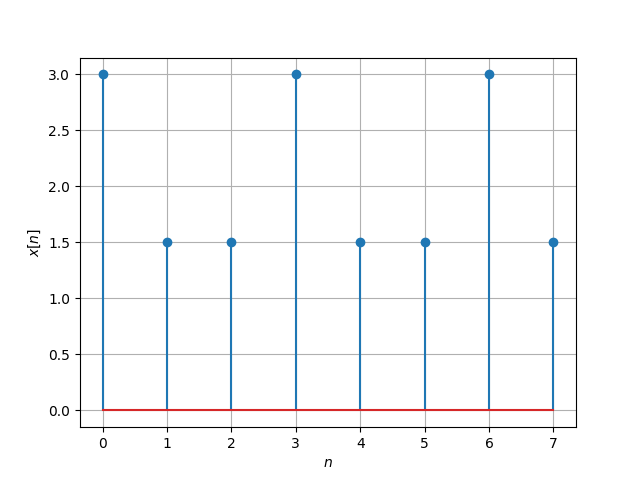
\includegraphics[width=\columnwidth]{figs/plot.png}
	\caption{Stem Plot of $x[n]$}
	\label{fig:plot_ee49}
\end{figure}
\end{document}
